\chapter{Problemanalyse}
\textit{I dette kapitel analyseres problemstillinger, som opstår i forbindelse med lægemiddelskift, og hvordan disse problemstillinger kan forebygges. Problemstillingerne vil sammenfattes i en opsummering og afsluttes med en problemformulering, der fremadrettet danner grundlaget for rapporten.}

\section{Lægemiddelskift}
Udgifterne til sygehusmedicin er stigende i flere lande, hvorfor flere lægemidler substitueres med henblik på at opnå besparelser på medicin~\citep{Ess2003,Johnston2011, Garcia2017}. Substitution af lægemidler medvirker til at et lægemiddel udskiftes til et andet lægemiddel og kan på baggrund af skiftet kategoriseres som generisk eller analog~\citep{DanskSelskabforPatientsikkerhed2009, Kairi2017}. Generisk substitution er substitution af lægemidler, der er  generisk ækvivalent med det forskrevne lægemiddel, herunder samme aktive stoffer, identiske styrke, koncentration og administrationsvej~\citep{DanskSelskabforPatientsikkerhed2009, Kairi2017, Lopes2012}. 
Analog substitution er substitution af alle lægemidler, som ikke er generiske~\citep{Kairi2017}. Disse afviger i sammensætningen men anses for at have sammenlignelige bivirkninger og terapeutiske egenskaber~\citep{DanskSelskabforPatientsikkerhed2009, Kairi2017}.


\section{Patientsikkerhedsmæssige konsekvenser} \label{sec:ProblemLaeg} 
Substitution kan lede til patientsikkerhedsmæssige konsekvenser~\citep{DanskSelskabforPatientsikkerhed2009}. En af årsagerne er, at producenter af lægemidler anvender forskellige hjælpestoffer, som på trods af kliniske forsøg, kan påvirke patienter forskelligt i forhold til optagelse og interaktion med andre lægemidler~\citep{Kairi2017}. Lægemidlet, som erstattes, kan have en anderledes form, størrelse eller farve end det forskrevne lægemiddel, hvormed patienten kan undlade at tage medicinen på grund af mistanke om fejl ved ordination~\citep{Kairi2017}. 

I Danmark er problemstillingerne vedrørende lægemiddelskift ikke belyst via videnskabelige studier, hvormed kendskab til de patientsikkerhedsmæssige konsekvenser er begrænset. Et norsk studie har undersøgt konsekvenserne ved generisk substitution~\citep{Hakonsen2010}, hvilket forventes at kunne relateres til Danmark. Interview med 100 sygeplejersker påviste, at fejlmedicinering opstod ved generiske lægemiddelskift~\citep{Hakonsen2010}. Ud af disse følte 
91~\% af sygeplejerskerne, at risikoen for fejl øges ved dispensering af generiske lægemidler, og 42~\% oplevede fejl som følge af generisk substitution~\citep{Hakonsen2010}.
Typer af medicineringsfejl ved generisk substitution fremgår af Figur \ref{fig:GeneriskSubstitution} og årsagerne hertil er rapporteret af 42 sygeplejersker~\citep{Hakonsen2010} og fremgår af Figur \ref{fig:GeneriskSubstitution1}.

\begin{figure}[H]\centering	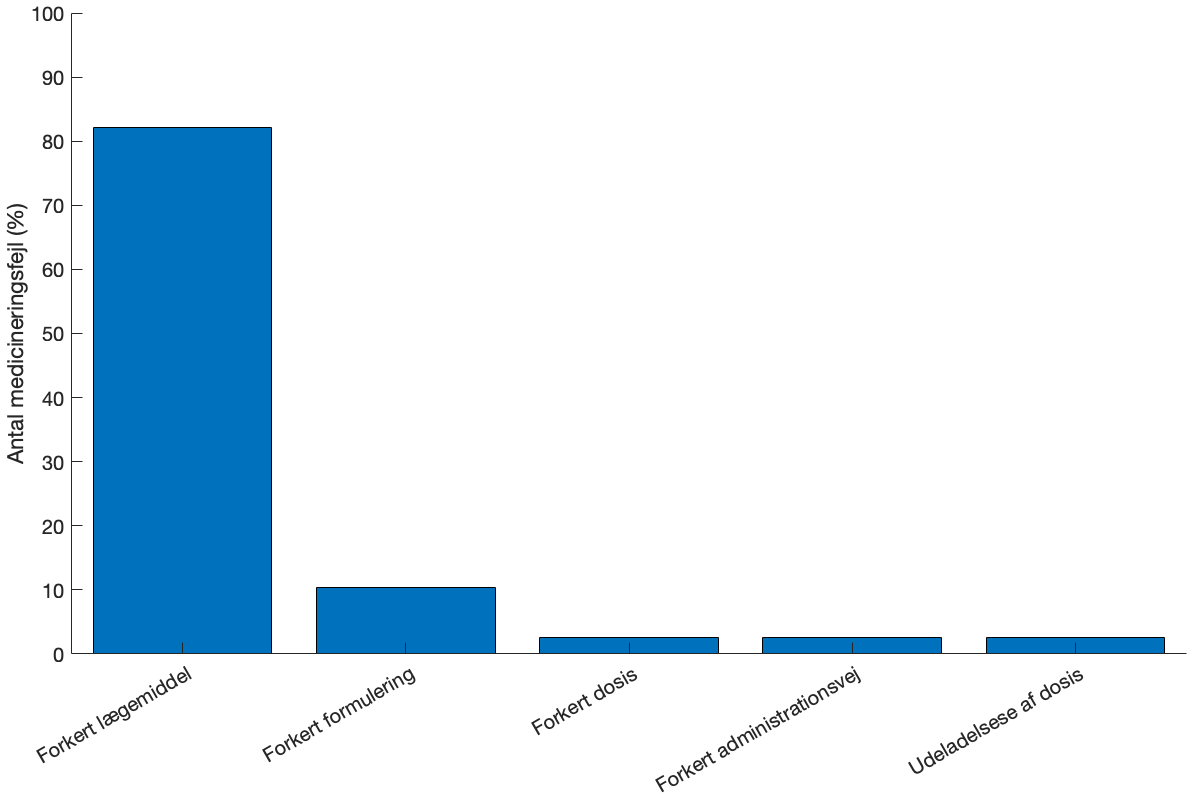
\includegraphics[width=0.9\textwidth]{billeder/GenSubb.png} 
	\caption{Typer af medicineringsfejl ved generisk substitution angivet i procent (n=100)~\citep{Hakonsen2010}.}
	\label{fig:GeneriskSubstitution}  
\end{figure}
\vspace{-0.5cm}

Det fremgår af Figur \ref{fig:GeneriskSubstitution}, at  størstedelen af fejlmedicinering ved generisk substitution skyldes forkert lægemiddel, hvoraf en mindre del skyldes formulering og i sjældnere tilfælde dosis, administrationsvej og udeladelse af dosis. Forkert lægemiddel sker ved dispensering eller administration af et andet lægemiddel end det forskrevne. Forkert formulering sker, fordi lægemidlets fysiske form er ændret f.eks. fra tabellet til smeltetabellet. Forkert dosis er relateret til forkert mængde af lægemidlet og administrationsvej er forkert indtagelse af lægemidlet. 

\vspace{-0.2cm}
\begin{figure}[H]\centering	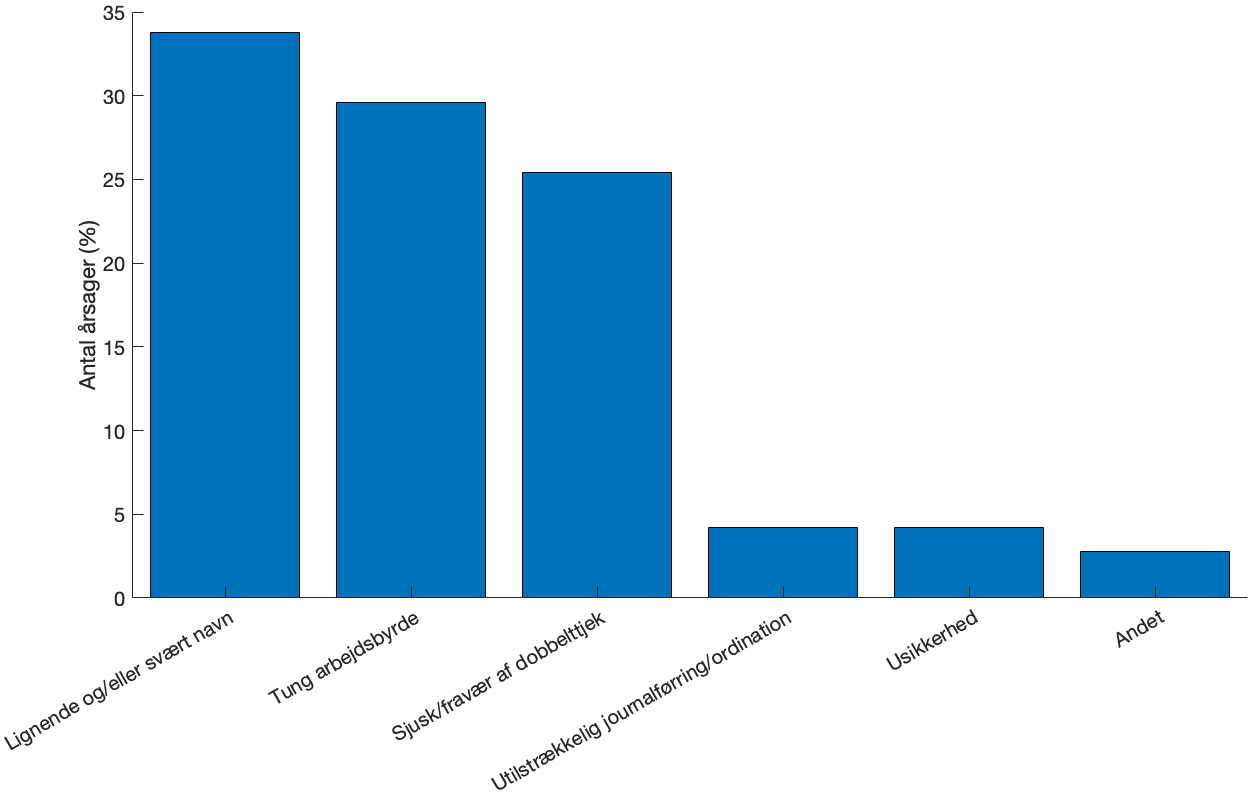
\includegraphics[width=0.9\textwidth]{billeder/GenSubbb.png} 
	\caption{Årsager til medicineringsfejl ved generisk substitution angivet i procent (n=42)~\citep{Hakonsen2010}.}	\label{fig:GeneriskSubstitution1}  
\end{figure}
\vspace{-1cm}

Det fremgår af Figur \ref{fig:GeneriskSubstitution1}, at størstedelen af årsagerne til medicineringsfejl ved generisk substitution skyldes lignende og/eller vanskeligt lægemiddelnavn, tung arbejdsbyrde og sløvhed eller fravær af dobbelttjek. En mindre del skyldes utilstrækkeligt journalførring og/eller ordination, usikkerhed eller andet. 

%I USA skyldes 25~\% af medicineringsfejl look-a-like rapporteret af US Pharmacopoeia, som er en organisation, hvis formål er at forbedre global sundhed gennem offentlige standard og relatede programmer.~\citep{http://www.usp.org}. I en undersøgelse af
%400 dødsfald forårsaget af medicineringsfejl blev det påvist at 
%5\% af dødsfaldene blev henført til navnebeskyttet navn forvirring og 4\% til generisk navn forvirring foretaget af US Food and Drug Administration~\citep{Garcia2017}.
%
%Der er dog begrænset bevis for at generisk substitution forstyrrer patientsikkerheden, men flere tilfælde, hvor patienter indlægges på grund af overdoser forårsaget af indtagelse af to eller flere lægemidler med samme aktive stof med forskellige mærker er rapporteret.~citep{Garica2017}

I flere lande opstår forkert lægemiddel ofte i forbindelse med forvirring ved forveksling af lægemiddelnavne~\citep{DanskSelskabforPatientsikkerhed2009}, hvilket afspejles i det norske studie. Forveksling af navn kan f.eks. forekomme ved Panodil, som er et smertestillende lægemiddel, og Plendil, som anvendes til behandling af forhøjet blodtryk~\citep{DanskSelskabforPatientsikkerhed2009}. 
I et studie blev det påvist, at forkert lægemiddel i op til 5~\% af tilfældene medførte uønskede bivirkninger~\citep{Basco2010}, mens sjældnere tilfælde har medført forlænget indlæggelse, forværret sygdom eller dødsfald~\citep{DanskSelskabforPatientsikkerhed2009}.

En af årsagerne til medicineringsfejl er lignende lægemiddelnavne, såkaldte look-a-likes. Disse lægemidler har ortografiske eller fonetiske ligheder, hvilket vil sige at de er forholdsvis ens i skrive- eller talemåde~\citep{Garcia2017,Basco2016}. Et eksempel på ortografisk lighed er f.eks. Nitroglycerin og Nitrofurantoin, mens et eksempel på fonetisk lighed er Dopamin og Dobutamin~\citep{Basco2016}. Look-a-likes kan give anledning til at sundhedspersonalet utilsigtet bytter om på lægemidlerne~\citep{Lopes2012}, hvormed medicineringsfejl ved ordination, dispensering eller administration kan forekomme~\citep{Garcia2017,Lopes2012}. Derudover er det påvist, at sandsynligheden for fejl stiger ved antallet af ortografiske ligheder mellem to lægemidler~\citep{Basco2010}. 
Forvirringen kan ligeledes opstå ved forskellige suffiks eller præfiks, som kan give anledning til fejl i dispensering, såsom Efexor kontra Efexor Depot~\citep{DanskSelskabforPatientsikkerhed2009}. Samtidig kan brugen af forkortelser ved f.eks. dispenseringsformer give anledning til forveksling~\citep{Wittich2014}.

I det norske studie pointerede nogle af sygeplejerskerne, at forvirringen over at finde den korrekte substitution kunne give anledning til at doseringen og formuleringen var skyld i medicineringsfejl~\citep{Hakonsen2010}. Dette kan skyldes kognitive forstyrrelser hos sundhedspersonalet på grund af den tunge arbejdsbyrde~\citep{Wittich2014}. Samtidig kan forvirringen over ændring i lægemidlets placering og den hyppige udskiftning af lægemiddelleverandører, som sker ved substitution af lægemidler, medvirke til fejlmedicinering~\citep{Wittich2014}.

Medicinering var den hyppigste årsag til rapportering af utilsigtede hændelser i Danmark i år 2013~\citep{Patientombuddet2013}. Antallet af rapporteringer i Region Nordjylland er steget med over 36~\% fra år 2012 til 2014~\citep{Jensen2014}. Ud af 824 rapporterede utilsigtede hændelser i år 2014 skyldes 97 \% medicinering, 86 \% administration af medicin og 41 \% disponering~\citep{Jensen2014}, hvor mere end én rapporteret utilsigtede hændelser skyldes én eller flere grunde. Fælles årsager for medicineringsfejl ved ordination, administration, ordination og administration er i flere studier  forkert dosis og lægemiddel samt udeladelse af ordination, dispensering og administration af lægemidlet~\citep{Barker2002,Sundhedsstyrelsen2005,Lisby2005, Tully2009}.
Derudover er det påvist, at 23~\% af de europæiske indbyggere har været udsat for medicineringsfejl og at 18~\% af disse har medført alvorlige fejl, hvoraf det antages at mellem 50 og 70~\% kunne være forebygget~\citep{Garcia2017}. Dette kan skyldes manglende teknologier til at reducere og forebygge fejl, hvortil det forventes, at nogle medicinerinsfejl kan forebygges ved simple handlinger foretaget af farmaci industrien~\citep{Lopes2012}.
%Størstedelen af fejl forekommer i forbindelse med ordination og administration, hvoraf en mindre andel sker ved transskribering og dispensering~\citep{Agrawal2009, Anderson2002}. Gentagne årsager i disse studier var forkert dosis og lægemiddel samt udeladelse af ordination, dispensering og administration af lægemidlet~\citep{Barker2002,Sundhedsstyrelsen2005,Lisby2005, Tully2009}.

\section{Risikovurderingen af lægemiddelskift} \label{sec:ImpLaeg}
For at forebygge medicineringsfejl og derved forbedre patientsikkerheden vurderer SRN de enkelte lægemiddelskift før implementering i klinikken. Dele af risikovurderingen er tidskrævende, personafhængig og sårbar. Flere dele af processen, som foretages manuelt, kan gøres computerbaseret, hvormed processen vil blive mere effektiv, mindre sårbar og personafhængig. Samtidigt er dele af vurderingen erfaringsbaseret og stiller krav til den enkelte medarbejderes viden inden for området, hvormed det ikke er muligt at gøre denne del af vurderingen automatiseret.

SRN informerer ud fra risikovurderingen de enkelte hospitalsafdelinger i regionen omkring lægemiddelskift og uddyber information om lægemiddelskift, som er vurderet til at kræve særlig opmærksomhed ved implementering. Inden informationen sendes ud til klinikken gennemgås forskellige processer, som fremgår af Figur \ref{fig:Proces}, i forhold til at vurdere det enkelte lægemiddelskift ud fra forskellige faktorer, som har betydning for hvor kompleks implementering af lægemiddelskiftet er. 

\begin{figure}[H]\centering	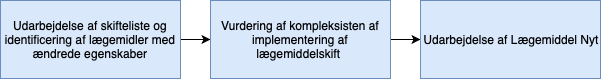
\includegraphics[width=1\textwidth]{billeder/proces.png} 
	\caption{Oversigt over processer, som gennemgås ved risikovurdering af lægemiddelskift inden implementering af disse i klinikken.}\label{fig:Proces}  
\end{figure}

Af Figur \ref{fig:Proces} fremgår det, at det første trin i processen omhandler udarbejdelse af skifteliste og identificering af faktorer, som er ændret ved lægemidlet. Dette sker ved sammenligning af egenskaber for lægemidlet fra foregående år med året for skiftet i forhold til ændringer. Formålet med skiftelisten, materiale der anvendes og faktorer som identificeres fremgår af Tabel \ref{table:Proces}. Ændring i lægemidlets egenskaber, markeres manuelt og angives som en bemærkning af én medarbejder fra SRN, ud fra fremgangsmåden som er yderligere beskrevet af Appendiks \ref{App:Skiftelister}.

Når skiftelisten er udarbejdet anvendes denne til at vurdere kompleksiteten af implementering af lægemiddelskift, som er den næste proces illustreret af Figur \ref{fig:Proces}. Lægemiddelskift vurderes af medarbejdere fra SRN, som er ansvarlige for hvert deres Anatomisk Terapeutisk Kemisk (ATC) område, ud fra ændringer, der er markeret i skiftelisten og en skabelon til implementering af lægemiddelskift. Formålet og eksempler på faktorer som vurderes i denne proces er beskrevet af Tabel \ref{table:Proces} samt yderligere beskrevet af skabelon til implementering af lægemiddelskift, som fremgår af Appendiks \ref{App:Skabelon}.

Ud fra skiftelisten og vurdering af implementering af lægemiddelskift informeres hospitalsafdelingerne via Lægemiddel Nyt, hvilket fremgår af Figur \ref{fig:Proces} som den sidste proces. Lægemiddel Nyt indeholder oplysninger om lægemiddelskift, der indgår i Regions Nordjyllands rekommendationsliste, som er bestemt af Lægemiddelkomitéen~\citep{RegionNordjylland2018}, og hospitalsafsnittenes standardsortimenter. Formålet og faktorer som vurderes i udarbejdelsen af Lægemiddel Nyt fremgår af Tabel \ref{table:Proces}. Udover at informere om ændringer i lægemidlets egenskaber såsom navn, fremgår uddybende informationer, hvis lægemiddelskiftet f.eks. har medført ændringer i styrke, dispenseringsform eller udseende, hvilket kan ses illustrationer på i Lægemiddel Nyt fra år 2018, som fremgår af Appendiks \ref{App:LaegemiddelNyt}. 

\begin{table}[H]
\caption{Procesbeskrivelse af skifteliste, vurdering af kompleksiteten af implementering af lægemiddelskift og Lægemiddel Nyt.} 
\label{table:Proces}
\begin{tabular}{|p{1.8cm}|p{3.5cm}|p{3.5cm}|p{4.2cm}|} \hline
\cellcolor[HTML]{C0C0C0}\textbf{} & \cellcolor[HTML]{C0C0C0}\textbf{Skifteliste} & \cellcolor[HTML]{C0C0C0}\textbf{Vurdering} & \cellcolor[HTML]{C0C0C0}\textbf{Lægemiddel Nyt}\\ \hline
\cellcolor[HTML]{C0C0C0}\textbf{Formål} & Identificering af ændrede egenskaber ved lægemidlet fra foregående år til året for skift. & Vurdering af kompleksiteten af implementering af lægemiddelskift. & Informere klinikken om ændringer i lægemidlets egenskaber og hvilke lægemiddelskit der kræves særligt opmærksomhed. \\ \hline
\cellcolor[HTML]{C0C0C0}\textbf{Materiale} & Fremgangsmåde for udarbejdelse af skifteliste. & Skifteliste  og skabelon til implementering af lægemiddelskift. & Skifteliste og materiale udarbejdet ved vurdering af kompleksiteten af implementering af lægemiddelskift. \\ \hline
\cellcolor[HTML]{C0C0C0}\textbf{Faktorer} & \vspace{-0.2cm}\begin{itemize}[topsep=-0.5cm,leftmargin=0.3cm] \item Navn \item Styrke\item Dispenseringsform \item Pakningsstørrelse \end{itemize} & \vspace{-0.2cm}\begin{itemize}[topsep=-0.5cm,leftmargin=0.3cm] \item Tidspunkt for skift\item Skiftets betydning for f.eks. klinikken \item Type af skift f.eks. forårsager ændringer ved skift i device \end{itemize}  & \vspace{-0.2cm}\begin{itemize}[topsep=-0.5cm,leftmargin=0.3cm] \item Navn \item Styrke \item Dispenseringsform \item Pakningsstørrelse \item Opbevaringsbetingelse \item Analog substitution  \end{itemize} \\ \hline  
\end{tabular}
\end{table} 

\section{Informationssystemer til risikovurdering} \label{sec:Inform_Risk}
Ingen videnskabelig litteratur har undersøgt, hvordan informationssystemer kan anvendes til vurderingen af lægemiddelskift inden implementering i klinikken. Den nuværende proces foregår manuelt, hvilket gør den tidskrævende, sårbar, og personafhængig, som beskrevet i Afsnit \ref{sec:ImpLaeg}. Informationssystemer er, modsat den menneskelige evne, i stand til at organisere og identificere sammenhænge mellem informationer fra en større mængde af data~\citep{Agrawal2009}, hvormed den nuværende vurdering af lægemiddelskift kan gøres mere ensartet og flere faktorer, som gør lægemiddelskift kompleks at implementere, kan vurderes. Dette vil understøtte beslutningsgrundlaget og samtidig gøre processen mindre personafhængig. Derudover kan dele af vurderingen som f.eks. identificering af ændringer ved lægemidlets egenskaber automatiseres, hvilket gør processen mindre sårbar. 

Flere studier har påvist, at informationssystemer er anvendelige i klinikken til forebyggelse af fejlmedicinering~\citep{Agrawal2009,  Stenner2010, Fischer2008, Simpson2008, Kaushal2002, Bates2000a}. Computerbaserede ordineringssystemer anvendes til at strukturere ordre, gøre disse letlæselige og fuldkommen samt gøre nødvendige oplysninger tilgængelige for klinikeren~\citep{Agrawal2009,Bates2000a}. I kombination med beslutningsstøtte, som f.eks. interaktion mellem lægemidler og automatisk beregning af styrke ved ændring i denne~\citep{Agrawal2009}, har computerbaserede ordineringssystemer påvist at være effektive i forbedringen af patientsikkerheden~\citep{Agrawal2009, Bates2000a}. Risikovurdering er bredt anvendt inden for sundhedsdomænet som beslutningsstøtte~\citep{Geissert2018, Rawshani2018,Barbar2010}. Disse studier anvender risikovurderingen som beslutningsstøtte ved udvikling af modeller til forudsigelse af sandsynligheden for, at patienter er i højrisiko for at få en overdoseringsrelateret indlæggelse og død ved opioder~\citep{Geissert2018} eller identificeringen af indlagte medicinske patienter i risiko for venøs tromboembolisme~\citep{Barbar2010}.

Til udvikling af en model til risikovurdering kan statistiske eller deterministiske metoder anvendes afhængig af problemstillingen~\citep{Boyko1990,Kirchsteiger1999}. Anvendes en statistisk metode til udvikling af et system til risikovurdering af lægemiddelskift vil skiftelister, som udarbejdes ved lægemiddelskift, være inputs variabler. Output variabler vil være de enkelte lægemiddelskift, som er kategoriseret på baggrund af registrerede patientsikkerhedsmæssige konsekvenser ved skiftet. Et eksempel på en statistisk metode er support vector machines~\citep{Koivu2018}, der udvikler en model på baggrund af et træningssæt til at forudsige, hvilken kategori et nyt lægemiddelskift tilhører. Da der både anvendes data til at udvikle og teste modellen, kræver denne metode en stor mængde af data. Ved anvendelse af en deterministisk metode til risikovurdering af lægemiddelskift vil skiftelister, som udarbejdes ved lægemiddelskift, være input variabler, mens output er baseret på et sæt af regler som er defineret på forhånd. Regelbaserede systemer består af regler, som er defineret helt eller delvist af en ekspert inden for området~\citep{Crina2008}. Da eksisterende viden inden for lægemiddelskift området, processerne for risikovurdering er kendte og data er begrænset kan et regelbaseret system anvendes til risikovurdering af lægemiddelskift. 

\section{Opsummering}
Lægemiddelskift sker for at begrænse udgifterne til sygehusmedicin, hvilket medfører substitution af lægemidler ~\citep{Ess2003, Johnston2011}. Substitution af lægemidler og implementeringen af disse i klinikken har betydning for forebyggelsen af medicineringsfejl og derved forbedring af patientsikkerheden, jævnfør Afsnit \ref{sec:ProblemLaeg}. Den nuværende vurdering af kompleksiteten af lægemiddelskift inden implementering i klinikken foregår manuelt, hvilket gør den tidskrævende og sårbar, som beskrevet i Afsnit \ref{sec:ImpLaeg}. Ligeledes er dele af vurderingen erfaringsbaseret, hvilket gør den personafhængig.

%Der er ingen videnskabelig litteratur, som har undersøgt informationssystemers anvendelighed til at gøre den nuværende vurdering af lægemiddelskift mindre personafhængig og sårbar. 
Flere studier har imidlertid påvist, at informationssystemer kan anvendes til at reducere antallet af medicineringsfejl i klinikken~\citep{Agrawal2009, Stenner2010, Fischer2008, Simpson2008}, jævnfør Afsnit \ref{sec:Inform_Risk}. Computerbaserede systemer til beslutningsstøtte, der anvender risikovurdering inden for samme domæne er bredt anvendt~\citep{Geissert2018, Rawshani2018,Barbar2010, Koivu2018}. Da dele af vurderingen, der foregår manuelt, såsom sammenligning af ændrede egenskaber ved lægemidlet, er kendte og kan baseres på regler kan et regelbaseret system anvendes til risikovurdering af lægemiddelskift i forhold til at identificere, hvornår et lægemiddelskift er kompleks at implementere, med henblik på at gøre den nuværende proces mindre personafhængig og sårbar. 

\section{Problemformulering}
\textit{Hvilken anvendelighed har et regelbaseret system til risikovurdering af lægemiddelskift med henblik på at forbedre den nuværende vurdering af lægemiddelskift?}


